\documentclass{../Common/Structure/doc_pdf}
%
\usepackage{pgfgantt}
\usepackage{amsmath}
\usepackage{amsfonts}
\usepackage{amssymb}



\titleSubtitle{{\Huge\textit{Power EnJoy}}\\{\LARGE Project Plan Document}}{Version 1.0.0}
\pageHeader{Project Plan Document}

\newcommand{\fp}[4]{\itemBold{#1}\par#2\begin{center}$#3 \cdot #4$\end{center}}


\begin{document}
	\titleToc{}
  \chapter{Introduction}
  The class inspected is \textbf{ProductDisplayWorker}.\\
It belongs to the package \textit{org.apache.ofbiz.shoppingcart.production}\\
The class inheritance is the following:
\begin{verbatim}
java.lang.Object
  org.apache.ofbiz.order.shoppingcart.product.ProductDisplayWorker
  org.apache.ofbiz.order.shoppingcart.product.ProductPromoWorker
  org.apache.ofbiz.order.shoppingcart.product.ProductPromoWorker.ActionResultInfo
  org.apache.ofbiz.order.shoppingcart.product.ProductStoreCartAwareEvents
\end{verbatim}

This class is a part of the usage of a \textbf{Worker pattern}.
It consist in the creation of a \textit{Worker object} that perform operation on a
specific type, or different type, of object.
This patters is really helpfull in the maintenance and the writing of the code
because permit to split the object we want to manage and the operation on this
object in order to maintain a well-posed structure a smaller class in term of line of code.
In plus this class contains a private static class used into the method of \textbf{ProductDisplayWorker}.
Usually this pattern is used with another pattern called \textbf{Manager pattern}, in fact also in the this case, Apache OFBIZ, we find an Order Manager that
is charged all the payments.

\section{Class code}
For reader's convenience, the whole content of the \textbf{ProductDisplayWorker} Java class source file is reported below.
\lstinputlisting{./ProductDisplayWorker.java}

  \newpage

  \chapter{Function Points}
  The Functional Point approach is a technique that allows to evaluate the effort
needed for the design and implementation of a project. We have used this technique
to evaluate the application dimension basing on the functionalities of the
application itself. The functionalities list has been obtained from the RASD document
and for each one of them the realization complexity has been evaluated.
The functionalities has been groped in:
\begin{itemize}
\item Internal Logic File: it represents a set of homogeneous data handled by the system
\item External Interface File: it represents a set of homogeneous data used
by the application but handled by external application
\item External Input: elementary operation that allows input of data in the system
\item External Output: elementary operation that creates a bit stream towards
the outside of the application
\item External Inquiry: elementary operation that involves input and output operations
\end{itemize}

\newpage

The following table outline the number of Functional Point based on functionality
and relative complexity:

\begin{table}[h]
	\centering
	\begin{tabular}{| l | l | l | l |}
		\hline
		\multirow{2}{*}{\textbf{Function Type}} & \multicolumn{3}{c|}{\textbf{Complexity}} \\
		\cline{2-4}
		& Simple & Medium & Complex  \\
		\hline
		Internal Logic File & 7 & 10 & 15 \\ \hline
		External Interface File & 5 & 7 & 10 \\ \hline
		External Input & 3 & 4 & 6 \\ \hline
		External Output & 4 & 5 & 7 \\ \hline
		External Inquiry & 3 & 4 & 6 \\ \hline

	\end{tabular}
\end{table}


\section{Internal Logic File}
Internal Logic Files are homogeneous sets of data used and managed by the application.\\
Summary of the calculated weights:
\begin{equation*}
	\begin{aligned}
		&	FP_{ILF}
		& & = 5 \cdot w_{Simple,ILF} + 3 \cdot w_{Medium,ILF} + 1 \cdot w_{Complex,ILF}\\
		&&& = 5 \cdot 7 + 3 \cdot 10 + 1 \cdot 15\\
		&&& = 80\\
	\end{aligned}
\end{equation*}
In details:
\begin{itemize}
	\fp{Ride}{Ride data. Frequent modifications, frequent insertions, frequent readings.}{1}{w_{Medium,ILF}}
  \fp{User}{Personal Registered Passenger data. Infrequent modifications, but frequent insertions and readings.}{1}{w_{Medium,ILF}}
  \fp{Car}{Car information. Infrequent insertion and modification, frequent reading}{1}{w_{Medium,ILF}}
	\fp{Customer Service}{Customer help request. Very infrequent modifications, insertions and readings.}{1}{w_{Simple,ILF}}
	\fp{Payment}{Data of the ended rent. Infrequent modification and reading, very frequent insertion}{1}{w_{Complex,ILF}}
	\fp{Payment Method}{User's payment data, Frequent readings, infrequent modification and insertion}{1}{w_{Simple,ILF}}
	\fp{Parking}{Parking data, frequent reading, infrequent insertion and modifications}{1}{w_{Simple,ILF}}
	\fp{Service Station}{Service station data. frequent reading, infrequent insertion and modifications}{1}{w_{Simple,ILF}}
	\fp{GPS Data}{GPS Data, Database Server side. Very frequent insertions and readings, but very infrequent modifications.}{1}{w_{Simple,ILF}}
\end{itemize}
%
\section{External Interface File}
External Interface Files are homogeneous sets of data used by the application but generated and maintained by other applications.\\
Summary of the calculated weights:
\begin{equation*}
	\begin{aligned}
		&	FP_{ELF}
		& & = 2 \cdot w_{Simple,ELF}\\
		&&& = 2 \cdot 5\\
		&&& = 10\\
	\end{aligned}
\end{equation*}
\newpage{}
In details:
\begin{itemize}
\fp{Google Maps API}{Google Maps API related data about Travel Time and Addresses. Very frequent readings.}{1}{w_{Simple,ELF}}
\fp{Paypal API}{Paypal API request related to user's payement. Frequent insertion}{1}{w_{Simple,ELF}}
\end{itemize}
%
\section{External Input}
External Inputs are elementary operations to elaborate data coming from the external environment.\\
Summary of the calculated weights:
\begin{equation*}
	\begin{aligned}
		&	FP_{EI}
		& & = 5 \cdot w_{Simple,EI} + 2 \cdot w_{Medium,EI} + 2 \cdot w_{Complex,EI}\\
		&&& = 5 \cdot 3 + 2 \cdot 4 + 2 \cdot 6\\
		&&& = 35\\
	\end{aligned}
\end{equation*}
In details:
\begin{itemize}
	\fp{Login}{This operation requires a simple effort. In fact it has to perform few steps in order to conclude the procedure.}{1}{w_{Simple,EI}}
	\fp{Logout}{This operation requires a simple effort. In fact it has to perform few steps in order to conclude the procedure.}{1}{w_{Simple,EI}}
	\fp{Registration}{This operation requires a simple effort. In fact it has to perform few steps in order to conclude the procedure.}{1}{w_{Simple,EI}}
	\fp{Handle Personal Profile}{This operation requires a simple effort. In fact it has to perform few steps in order to conclude the procedure.}{1}{w_{Simple,EI}}
	\fp{Car Interaction}{This operation requires a medium effort. In fact it is very frequent.}{1}{w_{Medium,EI}}
	\fp{Car Reservation}{This operation requires a complex effort. In fact it has to perform many elementary steps in order to handle it}{1}{w_{Complex,EI}}
	\fp{Problem}{This operation requires a medium effort}{1}{w_{Medium,EI}}
  \fp{Rent}{This operation requires a simple effort.}{1}{w_{Simple,EI}}
  \fp{End of Rent}{This operation requires a complex effort. In fact it has to perform many elementary steps in order to handle it}{1}{w_{Complex,EI}}
\end{itemize}
%
\section{External Output}
External Outputs are elementary operations that generate data for the external environment, and they usually include the elaboration of data from logic files.\\
Summary of the calculated weights:
	\begin{equation*}
		\begin{aligned}
		&	FP_{EO}
		& & = 4 \cdot w_{Simple,EO}\\
		&&& = 4 \cdot 4\\
		&&& = 16\\
	\end{aligned}
\end{equation*}
In details:
\begin{itemize}
	\fp{User Notification}{The result of the end of the rent must be send to the user who handle it}{1}{w_{Simple,EO}}
	\fp{Email Confirmation}{The result of this operation must be sent to the user that registers}{1}{w_{Simple,EO}}
	\fp{Maintenance Notification}{The result of the maintenance call must be sent to the specific user.}{1}{w_{Simple,EO}}
	\fp{Reservation}{Informations about the reservation must be sent to the related user}{1}{w_{Simple,EO}}
\end{itemize}
%
\section{External Inquiry}
External Inquiries are elementary operations that involve input and output, without significant elaboration of data from logic files.\\
Summary of the calculated weights:
\begin{equation*}
	\begin{aligned}
		&	FP_{EIQ}
		& & = 2 \cdot w_{Medium,EIQ}\\
		&&& = 2 \cdot 4\\
		&&& = 8\\
	\end{aligned}
\end{equation*}
In details:
\begin{itemize}
	\fp{Manager car status}{In order to perform these operations the system has to retrieve, send and render simple data.}{1}{w_{Medium,EIQ}}
	\fp{Manager user status}{In order to perform these operations the system has to retrieve, send and render simple data.}{1}{w_{Medium,EIQ}}
\end{itemize}
%
\section{Summary}
All the calculated $FP_{i}$ sums up to $FP$, which is the total Function Points value:
\begin{equation*}
	\begin{aligned}
		&	FP
		& & = FP_{ILF} + FP_{ELF} + FP_{EI} + FP_{EO} + FP_{EIQ}\\
		&&& = 80 + 10 + 35 + 16 + 8\\
		&&& = 149\
	\end{aligned}
\end{equation*}
The total $FP$ value is then multiplied by a constant factor $k_{i,j}$ that depends on the programming language $i$ used to develop the software and the company gearing ratio $j$.\par
The gearing ratio is the level of a company's debt related to its equity capital, usually expressed in percentage form.
Gearing is a measure of a company's financial leverage and shows the extent to which its operations are funded by lenders versus shareholders.\par
This final calculation gives us the number of SLOC $n_{SLOC}$ estimated for \PowerEnJoy{}:
\begin{equation*}
	\begin{aligned}
		&   n_{SLOC}
		& & = FP \cdot k_{Java, Avg}\\
		&&& = 149 \cdot 53\\
		&&& = 7897 \text{ SLOC}
	\end{aligned}
\end{equation*}
%


	\chapter{COCOMO}
	
This chapter describes the estimation achieved through COCOMO II: a complex, non linear model that takes in account the characteristics of the product, people and processes.
In order to generate the Constructive Cost Model we decided to use an online COCOMO II calculator on \url{http://csse.usc.edu/tools/COCOMOII.php}, using the  FP Sizing Method.
We also usedCOCOMO II - Model Definition Manual to make better choices of the parameters we had to insert into the  model.
\begin{itemize}
  \itemBold{Software Size}
    \begin{itemize}
      \itemBold{Unadjusted Function Points} The value FP has been taken as parameter, so 149 is the value chosen for this field.
      \itemBold{Language} The language of choice is Java, and not only Java EE, because the software is possibly a combination of different flavours of Java  (Java  SE, Java  EE and Java  for Android).
    \end{itemize}
  \itemBold{Software Scale Drivers}
    \begin{itemize}
      \itemBold{Precedentedness} Since we had a previous experience using Java SE for medium-size projects, but we have never used Java EE for developing such a big application we  decided to set this parameter to Nominal.
      \itemBold{Development Flexibility} Given that we had not strict specifications so we set this parameter to High.
      \itemBold{Architecture/Risk Resolution} Since we have designed several documents before the actual development, including this PPD, the development of the system to be has little chances of failing, so we choose  a  Nominal value.
      \itemBold{Team Cohesion} After a few days dedicated to create a efficient and fast workspace, the cohesion reached a Very High  level.
      \itemBold{Process Maturity} We understood, support and follow the process so we choose a High level for this parameter.
    \end{itemize}
  \itemBold{Software Cost Drivers}
    \begin{itemize}
      \item Product
        \begin{itemize}
          \item Required Software Reliability: Given that a failure in the software system could lead to moderate problems we choose Nominal level.
          \item Data Base Size:  Since we have a distributed application, the focus is on the lines of code instead of being on the size of the testing Database; so we choose a Low level parameter.
          \item Product Complexity: We made an average of the various complexity areas and we choose a High level parameter.
          \item Developed for Reusability:  We decided to develop reusable system components, so we came up with an High level parameter.
          \item Documentation Match to Lifecycle Needs: The standard level of documentation is required, so the chosen level is Nominal.
        \end{itemize}
      \item Personnel
        \begin{itemize}
          \item Analyst Capability: The personnel demonstrated a Nominal level of analysis ability.
          \item Programmer Capability: The personnel demonstrated efficiency working together as a team, so we chose High level for this  parameter.
          \item Personnel Continuity: The project will be developed always by the initial programmers, so the project’s annual personnel turnover is very low (7 % for year). For this reason we have chosen High for this parameter.
          \item Application Experience: Since the last time the development team has worked on a so complicated project was a year ago, we have chosen Nominal for this parameter.
          \item Platform Experience: The same as Application Experience ; we have chosen Nominal level for this parameter too.
          \item Language and Toolset Experience: The team is quite familiar with the development, analysis and design representation, so we choose High level for this parameter.
        \end{itemize}
      \item Platform
        \begin{itemize}
          \item Time Constraint: We have no relevant time constraints, so we choose Nominal level for this parameter.
          \item Storage Constraint: We have no relevant storage constraint, so we choose Nominal level for this parameter.
          \item Platform Volatility: Our hardware and software platforms will not change often, so we will have  no volatility and therefore we choose a Low level for this  constraint.
        \end{itemize}
      \item Project
        \begin{itemize}
          \item Use of Software Tools: The team is provided of a set of strong and mature life-cycle tools, moderately integrated one into each other.  So we choose an High level for this  parameter.
          \item Multisite Development: The team is in average fully collo- cated, so the chosen level is Nominal.
          \item Required Development Schedule: The project is not sub- jected on a particular constraint oppression, so we have chosen Nominal for this parameter.
        \end{itemize}
      \end{itemize}
    \itemBold{Maintenance} This value is set to Off
    \itemBold{Software Labour Rates}
      \begin{itemize}
        \item Cost per Person-Month (Dollars): We have chosen the average value of 1500\$/month for this parameter.
      \end{itemize}
    \end{itemize}


  \begin{center}
  	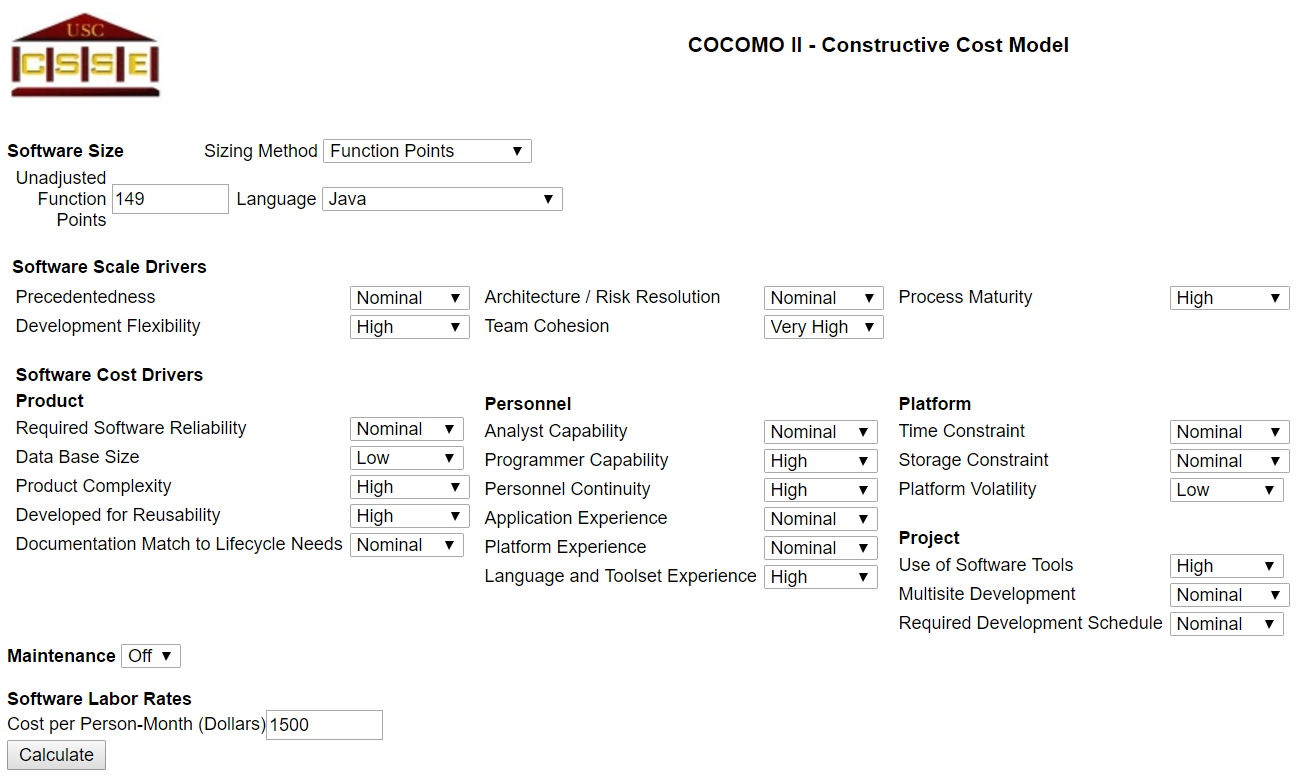
\includegraphics[width=\textwidth]{Resources/Cocomo_2.PNG}
    \captionof{figure}{COCOMO Parameters}
  	\label{COCOMO tools}
  \end{center}
  \newpage{}
  And here below we can see the result:

  \begin{center}
  	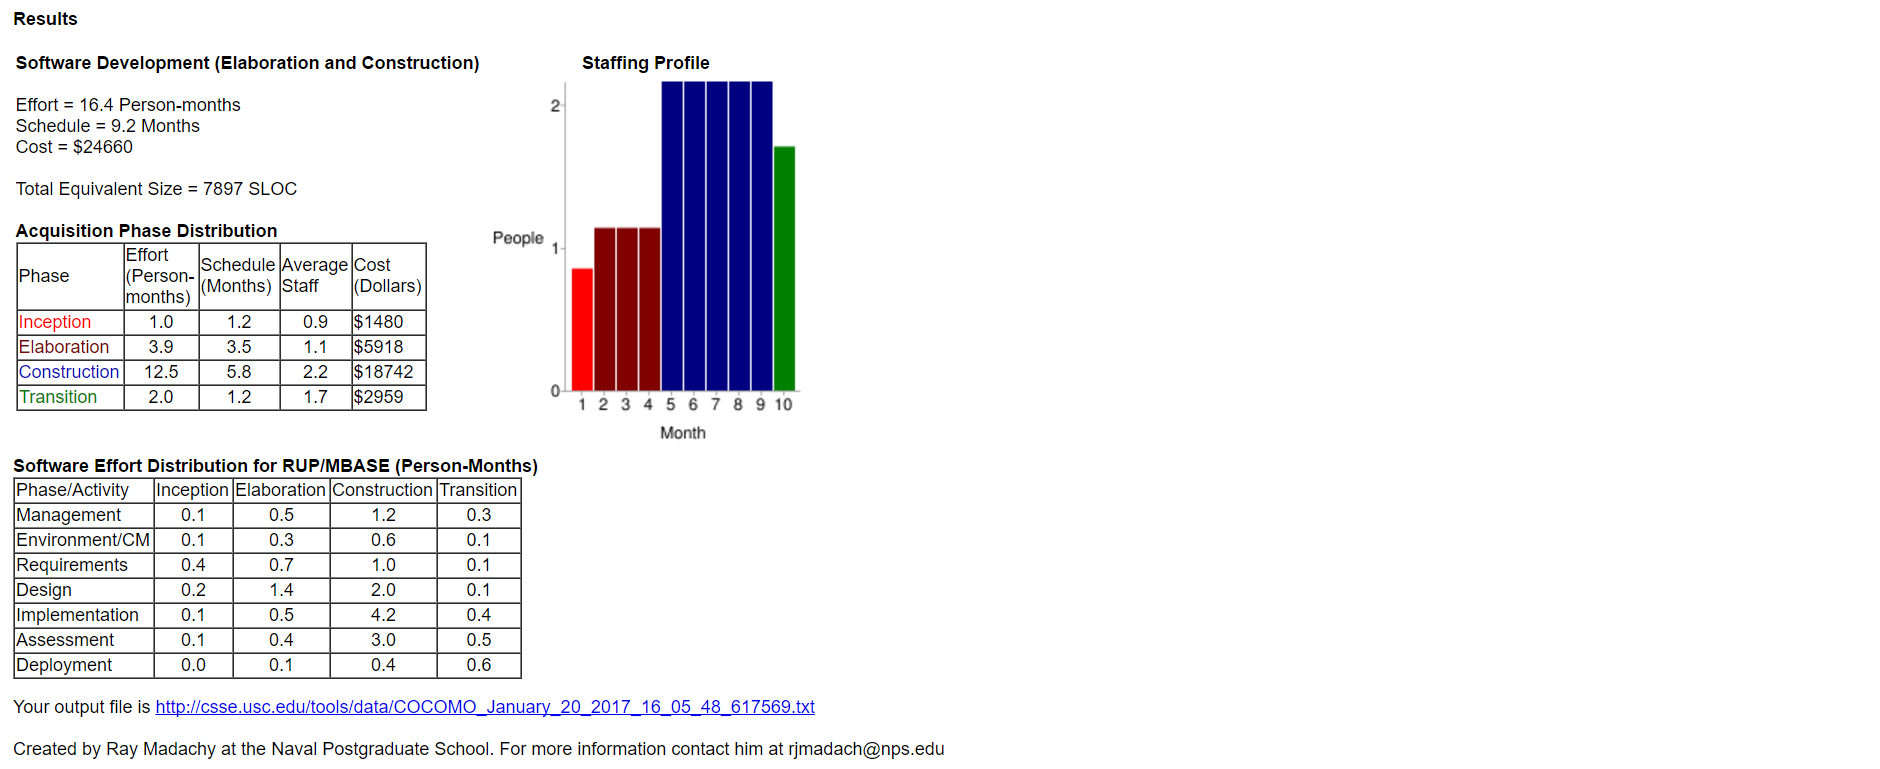
\includegraphics[width=\textwidth]{Resources/Cocomo_1.PNG}
    \captionof{figure}{COCOMO Results}
  	\label{COCOMO result}
  \end{center}

  \newpage

	\chapter{Task and Schedule}
	\section{Task}
Several tasks has been identified in our project. In the following table we can find three categories: one that labels the tasks, one for the description and the last one for the completion state to each task.

\begin{center}
	\begin{tabulary}{\linewidth\tymin=70pt}{Y{2cm}|Y{6cm}|Y{2.25cm}}
		\textbf{Task} & \textbf{Description} & \textbf{Completed?}\\ \hline
		T1a & RASD - Writing & Yes \\ \hline
		T1b & RASD - Presentation & Yes \\ \hline
		T2a & DD - Writing & Yes \\ \hline
		T2b & DD - Presentation & Yes \\ \hline
		T3 & ITPD - Writing & Yes \\ \hline
		T4 & PPD - Writing & Yes \\ \hline
		T5 & Implementation & No \\ \hline
		T6 & Unit Testing & No \\ \hline
		T7 & Integration Testing & No \\ \hline
		T8 & System Testing & No \\ \hline
		T9 & User Acceptance - Alpha Testing & No \\ \hline
		T10 & User Acceptance - Beta Testing & No \\ \hline
		T11 & Release To Market & No \\
	\end{tabulary}
\end{center}

\section{Schedule}
Below there are represented a table and a diagram that show how the time has been divided between the various phase of the software life cycle ; the result is then more clear in Gantt chart.
The table identifies:

\begin{itemize}
  \item The date in which the given task starts,
  \item The date in which the given task ends,
  \item The interval in [\textbf{day}] that separates the starting date from the ending date
\end{itemize}

\begin{center}
	\begin{tabulary}{\linewidth\tymin=70pt}{Y{1cm}|Y{3cm}|Y{3cm}|Y{1.7cm}}
		\textbf{Task} & \textbf{Start} & \textbf{End} & \textbf{Interval} \\ \hline
		T1a & 16/10/2016 & 13/11/2016 & 28\\ \hline
		T1b & 16/11/2016 & 16/11/2016 & 1\\ \hline
		T2a & 17/11/2016 & 11/12/2016 & 24\\ \hline
		T2b & 14/12/2016 & 14/12/2016 & 1\\ \hline
		T3 & 09/01/2017 & 15/01/2017 & 6\\ \hline
		T4 & 16/01/2017 & 22/02/2017 & 6\\ \hline
		T5 & 04/02/2017 & 30/05/2017 & 117\\ \hline
		T6 & 31/05/2017 & 29/06/2017 & 29\\ \hline
		T7 & 30/06/2017 & 28/07/2017 & 28\\ \hline
		T8 & 29/07/2017 & 29/08/2017 & 31\\ \hline
		T9 & 30/08/2017 & 27/09/2017 & 28\\ \hline
		T10 & 28/09/2017 & 26/10/2017 & 28\\ \hline
		T11 & 27/10/2017 & 27/10/2017 & 1\\
	\end{tabulary}
\end{center}

\section{Gant Diagram}
Here is built a Gantt Diagram showing the schedule chosen for \PowerEnJoy{} project tasks

\begin{center}
  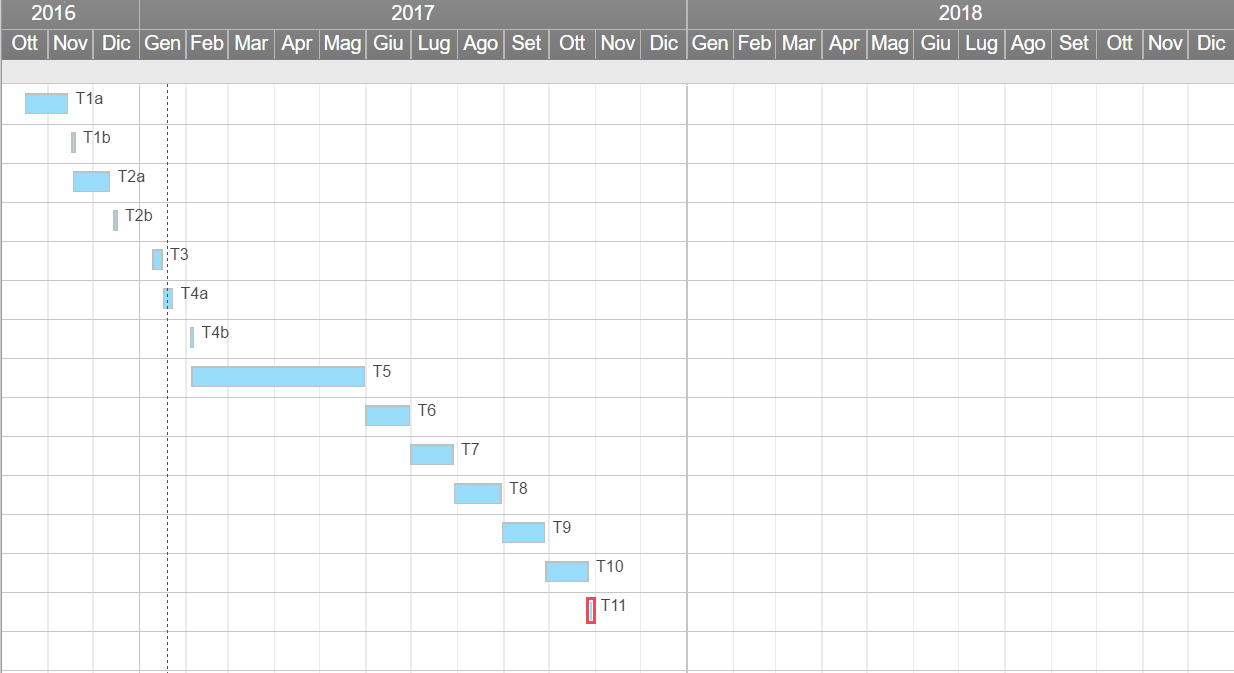
\includegraphics[width=\textwidth]{Resources/GanttDiagram.PNG}
  \captionof{figure}{Gant Diagram}
  \label{Gant Diagram}
\end{center}


	\chapter{Resources Allocation}
	This section covers the problem of allocating the human resources to each task in order to respect the identified scheduling.
We are a group of two people, and we do not have any kind of concurrency in the tasks that we identified, so we are going to work together on the same task at the same time during the whole duration of the project.
As shown before the project can be managed by more or less two people in nine months, and this respects the scheduling we devised.

\section{Staff Allocation Charts}
A chart is provided for the best visualization of the staff allocation.
For graphical issues, some consecutive tasks are merged one into the other.

\begin{center}
  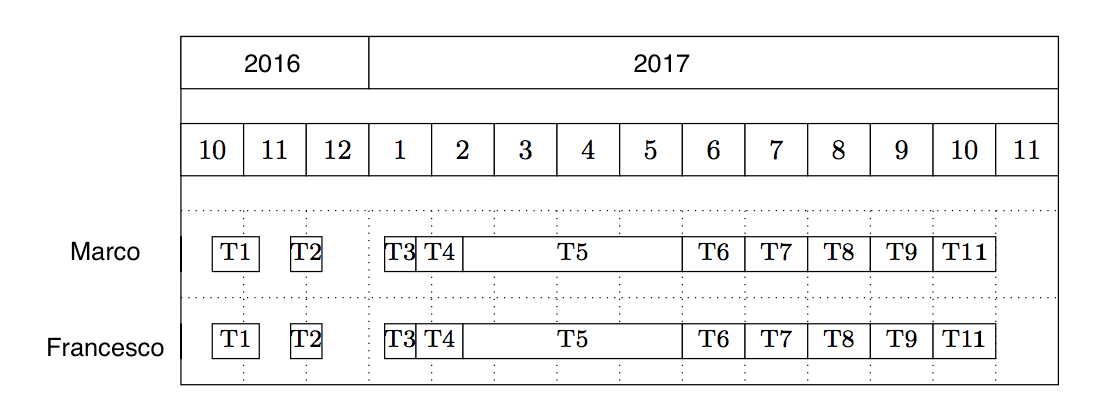
\includegraphics[width=\textwidth]{Resources/resources.png}
  \captionof{figure}{Staff allocation chart}
  \label{Staff allocation chart}
\end{center}


	\chapter{Risk}
	
The project is subject to a series of risks with different levels of danger.
In order to prevent so in necessary to have an \textbf{Proactive Risk Management Strategy} that could prevent or eventually solve some
of the major risk. In order to build a good \textbf{Proactive Risk Management Strategy} we describe in this chapter the potential risk
the project is subject to, categorysing them and proposing a solution for each main category. Business risk are not take into account
in this chapter as we presume an carefull analysis of the market, budget and business strategy has already be done taking in account also
the related risk.
\begin{itemize}
    \itemBold{Project Risk}
      \begin{itemize}
        \item The work force available is less than expected. It could be caused by developers’ lack of experience in programming and in project planning and management.
        it could potentially slow down the overall project development thus leading to the risk of an extension of some deadline. A solution for this problem could be,
        in scheduling phase, take into account that possibility and assign a bit more effort than needed to each task.
      \end{itemize}
    \itemBold{Technical Risk}
      \begin{itemize}
        \item Faults in reusable software components have to be repaired before these components are reused. It could be prevented by a
        develop strong unit tests, in fact, it reduces the error' probability and in the worst case the reparation time is minimized.
        \item The database and other external software components used in the system cannot process as many operations per second as expected. It could be due to
        a under-estimation of the city dimension or a bigger amount of users than expected. A possible solution could be over-estimate the operations throughput in order to choose the appropriate support infrastructure.
      \end{itemize}
\end{itemize}


  \appendix
  \chapter{Appendix}

  \section{Tools}
  \begin{itemize}
  	\itemBold{TeXstudio} \LaTeX{} editor used to write the document.
		\itemBold{COCOMO Tool II} at \url{http://csse.usc.edu/tools/COCOMOII.php} to estimate the project dimension.
  	\itemBold{StarUML} To draw Gant diagram and Resources allocation.\end{itemize}
  \section{Hours of work}
  In the following are listed the hours of work that each member of the group did:
  \begin{enumerate}
  	\item Marco Redaelli: 16 \emph{hours}
  	\item Francesco Zanoli: 16 \emph{hours}
  \end{enumerate}
  \section{Version History}
  In the following are listed the differences between versions:
  \begin{enumerate}
  	\itemBold{ 22/01/2017} First version
  \end{enumerate}

  \end{document}
